\documentclass[conference]{IEEEtran}
\IEEEoverridecommandlockouts

\usepackage{cite}
\usepackage{amsmath,amssymb,amsfonts}
\usepackage{graphicx}
\usepackage{textcomp}
\usepackage{xcolor}
\usepackage[utf8]{inputenc}
\usepackage[T1]{fontenc}
\usepackage[brazil]{babel}
\usepackage{booktabs}
\usepackage{url}

% Figuras geradas pelos experimentos (resultados/ ao lado de relatorio/)
% Pooled (57 regiões) tem prioridade; região única fica para os mosaicos ilustrativos.
\graphicspath{{../resultados/_pooled/}{../resultados/_pooled_blend_extra/}{../resultados/2970_3_SE/shift_consistency/}{../resultados/2970_3_SE/blend_compare/}}

\begin{document}

\title{Equivariância a Translação na Super-Resolução por Tiles:
Análise do Gerador Satlas e Estratégia Ótima de Junção}

\author{
\IEEEauthorblockN{Marcel Fernandes Gomes}
\IEEEauthorblockA{\textit{Programa de Pós-Graduação em Computação} \\
\textit{Universidade Federal do Rio Grande do Sul}\\
Porto Alegre, Brasil \\
marcelgfernandes@gmail.com}
}

\maketitle

\begin{abstract}
Modelos de super-resolução (SR) de imagens de satélite são aplicados, em grandes
áreas, por inferência em \textit{tiles} de tamanho fixo, mas com posição arbitrária.
Se o gerador fosse perfeitamente equivariante a translação, deslocar o conteúdo
físico dentro do tile deveria apenas deslocar a saída, sem alterar os valores na
região sobreposta entre duas inferências. Neste trabalho medimos empiricamente quanto
essa propriedade se quebra no gerador ESRGAN/\,\texttt{SSR\_RRDBNet} do Satlas, em
modo \emph{zero-shot} (pesos pré-treinados, sem retreino), sobre imagens Sentinel-2.
Comparando a saída SR do mesmo conteúdo com o tile deslocado por inteiros de pixel em
baixa resolução (LR), quantificamos a discordância na sobreposição por uma métrica de
auto-consistência (\textit{shift-consistency} PSNR/SSIM), que dispensa verdade de
campo. O protocolo, validado inicialmente em uma única região, foi \textbf{estendido a
57 regiões} geograficamente distintas do Sul do Brasil, agregando os resultados de forma
\emph{pooled} (média entre regiões). Observamos que a discordância é significativa e
\emph{cresce monotonicamente} à medida que a sobreposição se aproxima da borda do tile:
o PSNR de auto-consistência cai de $30{,}8$\,dB (90\% de sobreposição) para $24{,}7$\,dB
(3\%), e o SSIM de $0{,}85$ para $0{,}45$, com baixa dispersão entre regiões
($\pm1{,}2$\,dB). Um perfil de erro em função da distância à borda localiza a causa: a
diferença média decai de $10{,}1$\,DN na borda para ${\sim}2{,}0$\,DN no interior,
coerente com um campo receptivo que excede o tile somado ao \textit{zero-padding}. A
partir desse perfil derivamos máscaras de junção e comparamos estratégias de
\textit{blend}; entre as clássicas, a gaussiana reduz o excesso de gradiente nas costuras
de $1{,}30$ para $1{,}05$ (ideal $1{,}0$) e eleva o PSNR de referência de $25{,}3$ para
$34{,}4$\,dB, e estratégias adicionais (Poisson com Dirichlet, data-driven suavizado)
chegam a superá-la. Os resultados quantificam a quebra de equivariância formal das CNNs
em um gerador de SR real, mostram que o achado é \textbf{robusto entre regiões} e
fornecem uma recomendação prática de montagem de mosaicos sem costura.
\end{abstract}

\begin{IEEEkeywords}
super-resolução, equivariância a translação, shift-consistency, ESRGAN, junção de tiles,
blending, Sentinel-2, sensoriamento remoto
\end{IEEEkeywords}

% ===========================================================================
\section{Introdução}
% ===========================================================================
A super-resolução (SR) por aprendizado profundo tornou-se ferramenta padrão para
ampliar a resolução efetiva de imagens de satélite, viabilizando a extração de feições
finas (bordas de campos agrícolas, corpos d'água pequenos, estradas vicinais) a partir
de sensores de resolução moderada como o Sentinel-2 ($\sim$10\,m/px)~\cite{b_sr_survey}.
Em aplicações reais sobre grandes áreas, a inferência é feita por \textit{tiles}: a
cena é fatiada em janelas de tamanho fixo, cada janela é super-resolvida
independentemente e as saídas são remontadas em um mosaico.

Esse procedimento expõe uma tensão pouco discutida. O modelo é treinado e avaliado em
tiles de tamanho fixo, mas \emph{não fixa a posição} do tile sobre o terreno --- a
grade de fatiamento é arbitrária. Surge então a pergunta de pesquisa central:
\textbf{o gerador é equivariante a translação?} Se fosse, dois tiles que cobrem a mesma
porção física do terreno, porém deslocados entre si, deveriam produzir exatamente os
mesmos pixels na região que compartilham. Onde isso falha, a remontagem produz
\emph{artefatos de costura} nas junções entre tiles.

Camadas convolucionais são, por construção, equivariantes a translação; redes
convolucionais profundas, porém, perdem essa equivariância estrita por causa de
\textit{padding} e subamostragem~\cite{b_shiftinv}. Essa fragilidade já foi documentada
empiricamente (CNNs profundas degradam sob translações de poucos
pixels~\cite{b_azulay}) e motivou tanto arquiteturas equivariantes por
construção~\cite{b_gconv} quanto geradores \emph{alias-free}, que restauram a
equivariância em modelos generativos~\cite{b_aliasfree} e são particularmente
pertinentes aqui, por se tratar de um gerador adversarial (ESRGAN). Em classificadores
busca-se \emph{invariância} (o rótulo não deve mudar com a posição do objeto), ao passo
que num gerador de SR (mapa imagem$\to$imagem, sem \textit{pooling} global) a
propriedade desejável é a \emph{equivariância}. Este trabalho é uma verificação empírica
direta dessa ressalva em um gerador de SR de produção. Nossas contribuições são:
\begin{itemize}
  \item um \textbf{protocolo de medida de \textit{shift-consistency} sem verdade de
  campo}, baseado na auto-consistência entre duas inferências do mesmo conteúdo com o
  tile deslocado por inteiros de pixel LR;
  \item um \textbf{diagnóstico do efeito de borda} (um perfil de erro em função da
  distância à borda do tile) que localiza a não-equivariância e a atribui ao campo
  receptivo que excede o tile somado ao \textit{zero-padding};
  \item uma \textbf{estratégia de junção guiada pelos dados} e a comparação com
  \textit{blends} usuais por uma métrica de costura.
\end{itemize}

O escopo é restrito ao Sentinel-2, domínio de treino do Satlas~\cite{b_satlas}, para
evitar o confundimento de \textit{domain shift} multissensor. Trata-se de um estudo
\emph{zero-shot} (sem retreino). O protocolo foi validado primeiro em uma \emph{única
região} e, em seguida, \textbf{estendido a 57 regiões} geograficamente distintas; os
resultados reportados são \emph{pooled} (agregados entre regiões), o que permite avaliar
a \textbf{robustez} do achado e sua dispersão entre áreas.

% ===========================================================================
\section{Descrição do Problema}
% ===========================================================================
\subsection{Super-resolução por tiles e equivariância a translação}
O gerador do Satlas é \emph{multi-frame}: recebe $N$ imagens LR da mesma região, em
datas distintas, empilhadas como entrada de $3N$ canais em uma janela $32\times32$, e
produz uma única saída em alta resolução (HR) $128\times128$, com fator $s=4$,
explorando informação sub-pixel entre as datas. Denotando por $f$ o gerador e por
$T_\Delta$ um operador de translação por $\Delta$ pixels, a \textbf{equivariância a
translação} ideal exige
\begin{equation}
f(T_\Delta x) = T_{s\Delta}\, f(x),
\label{eq:equiv}
\end{equation}
isto é, deslocar a entrada de $\Delta$ pixels LR deveria deslocar a saída de $s\Delta$
pixels HR \emph{sem alterar os valores}. Na região $\Omega$ comum a duas inferências
deslocadas, os pixels físicos são os mesmos; sob \eqref{eq:equiv}, as duas saídas
coincidiriam em $\Omega$. A discordância observada mede o quanto $f$ se afasta da
equivariância formal das suas camadas convolucionais~\cite{b_shiftinv}.

\subsection{Fontes de não-equivariância no Satlas}
Identificamos as fontes e controlamos os confundimentos:
\begin{itemize}
  \item \textbf{Campo receptivo $\gg$ tile.} O \texttt{RRDBNet} tem $23$ blocos RRDB
  ($\sim$350 convoluções $3\times3$ com \textit{padding} ``same''), gerando um campo
  receptivo da ordem de centenas de pixels LR --- muito maior que o tile $32\times32$.
  \emph{Todo} pixel de saída ``enxerga'' a borda do tile e o \textit{zero-padding}
  associado; não existe interior verdadeiramente limpo. É a causa principal sob teste.
  \item \textbf{Upsampling \texttt{nearest} $\times$4.} A interpolação por vizinho mais
  próximo é equivariante para deslocamentos \emph{inteiros} em LR ($\Delta \to s\Delta$
  exato). Por isso \emph{todos} os deslocamentos do experimento são inteiros em pixels
  LR: assim o grid HR alinha sem reamostragem e o \textit{upsampling} é removido como
  fonte de erro.
  \item \textbf{Seleção de frames.} A escolha de quais cenas usar é fixada
  \emph{globalmente} (uma vez, deterministicamente, pelo critério de menor fração de
  \textit{nodata}), de modo que toda posição usa exatamente os mesmos frames; caso
  contrário, a diferença viria da \emph{entrada}, não do modelo.
\end{itemize}

% ===========================================================================
\section{Solução Proposta}
% ===========================================================================
\subsection{Arquitetura base (ESRGAN/RRDBNet)}
Usamos o gerador ESRGAN~\cite{b_esrgan} na variante \texttt{SSR\_RRDBNet} do
Satlas-SR~\cite{b_satlas_sr} (modelo treinado sobre o conjunto
SatlasPretrain~\cite{b_satlas}), com os pesos públicos \texttt{esrgan\_8S2.pth}
($N=8$ frames).
\textbf{Não há retreino}: todo o estudo é \emph{zero-shot}. A perda original de treino,
reproduzida aqui apenas como contexto, combina termo de pixel, perceptual e
adversarial,
\begin{equation}
\mathcal{L} = \mathcal{L}_{pix} + \lambda_p \mathcal{L}_{perc} + \lambda_a \mathcal{L}_{adv}.
\label{eq:loss}
\end{equation}
O termo perceptual~\cite{b_lpips} e o adversarial favorecem texturas plausíveis, mas
não impõem qualquer restrição de consistência entre posições de tile, o que motiva o
diagnóstico deste trabalho.

\subsection{Protocolo de medida da equivariância}
Constrói-se \emph{uma vez} o \textit{stack} LR fixo, reprojetando as $N$ cenas para um
único grid comum (EPSG:3857 a $9{,}555$\,m/px) para garantir alinhamento pixel-a-pixel.
Selecionam-se âncoras interiores sem \textit{nodata}. Para cada âncora e cada
deslocamento horizontal $\Delta$, roda-se SR no \textit{offset} $0$ e no \textit{offset}
$\Delta$; como $\Delta$ pixels LR correspondem a $s\Delta$ pixels HR exatos, a
sobreposição $\Omega$ contém os \emph{mesmos pixels físicos}. A discordância é medida
pelo PSNR de auto-consistência,
\begin{equation}
\text{scPSNR}(\Delta) = 10\log_{10}\!\frac{255^2}{\mathrm{MSE}\big(I^{SR}_0|_\Omega,\,I^{SR}_\Delta|_\Omega\big)},
\label{eq:scpsnr}
\end{equation}
reportando-se também SSIM~\cite{b_ssim}, MAE e RMSE em $\Omega$. Varia-se a sobreposição
de $100\%$ ($\Delta=0$, controle, em que $\Omega$ é o tile inteiro e a discordância deve
ser nula) até ${\sim}3\%$ ($\Delta=31$).

\subsection{Perfil de borda e blend ótimo}
Para localizar a não-equivariância, acumula-se a diferença absoluta média por coluna de
$\Omega$ em função da distância $d$ à borda de tile mais próxima, formando o perfil
$P(d)$. Esse perfil mede a confiabilidade local da saída: quanto maior $P(d)$, menos
confiável aquele pixel para a junção. Define-se então uma máscara de peso
\textit{data-driven} $w(d) \propto 1/P(d)$ e comparam-se as estratégias
\texttt{none}, \texttt{linear}, \texttt{cosine}, \texttt{gaussian} e \texttt{data} na
montagem de um mosaico real. A qualidade da costura é medida por
\begin{equation}
\mathrm{seam\_excess} = \frac{\text{gradiente médio nas linhas de junção}}{\text{gradiente médio global}},
\label{eq:seam}
\end{equation}
cujo valor ideal é $\approx 1$ (a junção não se distingue do conteúdo); complementa-se
com PSNR/SSIM contra um mosaico de referência por recorte central.

% ===========================================================================
\section{Resultados Experimentais}
\label{sec:resultados}
% ===========================================================================
\subsection{Configuração}
Inferência \emph{zero-shot} com \texttt{esrgan\_8S2.pth} (sem retreino) em GPU
Tesla V100-PCIE-32GB.\footnote{\textbf{Reprodutibilidade.} Código dos experimentos,
metadados das cenas (proveniência), AOIs vetoriais e todos os resultados (CSV e figuras)
estão em \url{https://github.com/MarcelFernandesCGEO/cmp620_trabalho_final}. Pesos e código
do gerador: \url{https://github.com/allenai/satlas-super-resolution}. Cenas Sentinel-2
(produto TCI) obtidas do Copernicus Data Space Ecosystem
(\url{https://dataspace.copernicus.eu}); os rasters não são redistribuídos, mas a
proveniência permite o redownload.} O protocolo foi validado primeiro em uma \textbf{região-piloto}
(tile MGRS \textbf{T22JDM}, Sul do Brasil; $8$ cenas Sentinel-2 TCI, datas entre
2025-10-10 e 2026-05-03) e, em seguida, \textbf{estendido a 57 regiões} geograficamente
distintas, cada uma com $8$ cenas Sentinel-2 TCI (produto RGB, 10\,m) recortadas a uma
AOI vetorial e reprojetadas a um grid comum a $9{,}555$\,m/px. Parâmetros por região:
\texttt{tile}$=32$, $s=4$, $N=8$, âncoras interiores sem \textit{nodata} e
$\Delta \in \{0,3,6,10,13,16,19,22,26,29,31\}$ px LR (sobreposição de $100\%$ a
$3{,}1\%$). Os resultados a seguir são \emph{pooled} (a média entre as 57 regiões),
com a dispersão (desvio-padrão) entre regiões reportada quando relevante. Esse desenho
amplia substancialmente a quantidade de dados em relação à validação de região única
inicial e permite aferir a robustez do achado.

\subsection{Consistência sob deslocamento}
A Tabela~\ref{tab:consistency} e a Fig.~\ref{fig:consistency} resumem o resultado
central. No controle ($\Delta=0$) a discordância é nula (scPSNR $\approx 100$\,dB,
SSIM $=1{,}000$), validando o protocolo. Para qualquer deslocamento, porém, as duas
saídas \emph{divergem} (Fig.~\ref{fig:example}), e a divergência cresce de forma monotônica à medida que a
sobreposição encolhe --- ou seja, à medida que a região comparada se aproxima das
bordas dos tiles. Entre $90\%$ e $3\%$ de sobreposição, o scPSNR cai de $30{,}8$ para
$24{,}7$\,dB e o SSIM de $0{,}85$ para $0{,}45$, com o MAE subindo de $5{,}0$ para
$12{,}4$\,DN. O comportamento é \textbf{consistente entre as 57 regiões}: a dispersão do
scPSNR fica em torno de $\pm1{,}2$\,dB em todas as faixas de sobreposição, indicando que
o achado é robusto e não um artefato de uma área específica. Nota-se que mesmo a $90\%$
de sobreposição (região predominantemente interior) a coincidência \emph{não} é perfeita,
coerente com a inexistência de interior limpo quando o campo receptivo excede o tile.
\textbf{O gerador não é equivariante a translação.}

\begin{table}[htbp]
\caption{Shift-consistency vs sobreposição (Sentinel-2, $N=8$; \emph{pooled}, média entre 57 regiões)}
\label{tab:consistency}
\begin{center}
\begin{tabular}{ccccc}
\toprule
\textbf{Overlap} & \textbf{scPSNR}$\uparrow$ & \textbf{SSIM}$\uparrow$ & \textbf{MAE}$\downarrow$ & \textbf{RMSE}$\downarrow$ \\
\midrule
100,0\% (controle) & 99,99 & 1,000 & 0,00 & 0,00 \\
90,6\% & 30,83 & 0,850 & 5,03 & 7,88 \\
81,2\% & 29,91 & 0,819 & 5,83 & 8,76 \\
68,8\% & 28,94 & 0,780 & 6,76 & 9,79 \\
59,4\% & 28,35 & 0,753 & 7,38 & 10,50 \\
50,0\% & 27,81 & 0,722 & 7,99 & 11,20 \\
40,6\% & 27,24 & 0,685 & 8,68 & 12,00 \\
31,2\% & 26,65 & 0,642 & 9,44 & 12,88 \\
18,8\% & 25,78 & 0,568 & 10,64 & 14,31 \\
9,4\% & 25,09 & 0,505 & 11,67 & 15,57 \\
3,1\% & 24,65 & 0,452 & 12,40 & 16,43 \\
\bottomrule
\end{tabular}
\end{center}
\end{table}

\begin{figure}[htbp]
\centerline{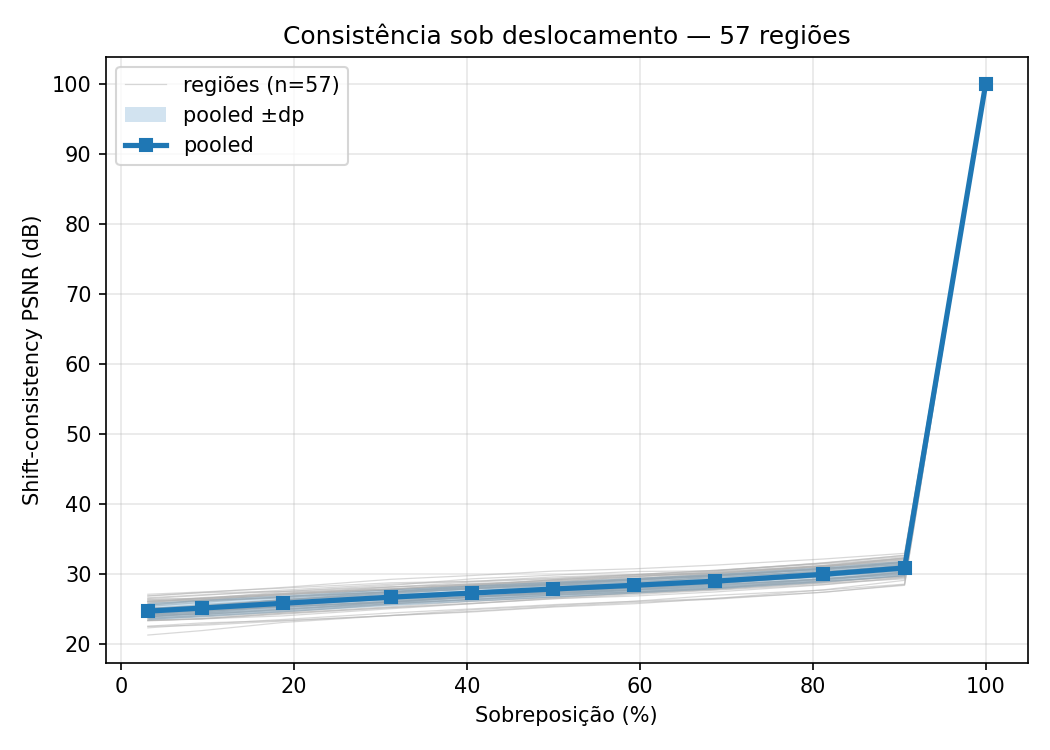
\includegraphics[width=\columnwidth]{fig_consistency_pooled.png}}
\caption{Consistência sob deslocamento (\emph{pooled}, 57 regiões). scPSNR (azul) e SSIM
(vermelho) em função da sobreposição, com a faixa de dispersão entre regiões. A queda
monotônica ao reduzir a sobreposição revela a não-equivariância; o salto a $100\%$
corresponde ao controle $\Delta=0$.}
\label{fig:consistency}
\end{figure}

\begin{figure}[htbp]
\centerline{
\includegraphics[width=\columnwidth]{fig_example.png}}
\caption{Exemplo qualitativo da não-equivariância (região-piloto T22JDM,
$\Delta=16$ px LR $\Rightarrow$ sobreposição de $50\%$). À esquerda e ao centro, as
saídas SR do \emph{mesmo} conteúdo físico com o tile em \textit{offset} $0$ e $16$ px
--- visualmente quase idênticas. À direita, a diferença absoluta (escala normalizada
$[0,1]$) na sobreposição: a discordância é não-nula e se \textbf{concentra junto às
bordas do tile} (topo e lateral direita) e ao longo de feições de alto gradiente (a
estrada, os limites de vegetação), coerente com o perfil de borda da
Fig.~\ref{fig:border}.}
\label{fig:example}
\end{figure}

\subsection{Onde a não-equivariância se concentra}
A Fig.~\ref{fig:border} mostra o perfil $P(d)$ \emph{pooled} (média entre as 57 regiões):
a diferença absoluta média é máxima \emph{na borda} do tile ($\sim$$10{,}1$\,DN em $d=0$)
e \emph{decai monotonicamente} para o interior, chegando a ${\sim}2{,}0$\,DN a
$\sim$50\,px de profundidade. Esse é o
diagnóstico que liga o achado à teoria: como cada pixel de saída integra o
\textit{zero-padding} da borda através de um campo receptivo que excede o tile, o erro
de equivariância é introduzido na borda e se atenua à medida que a influência relativa
do \textit{padding} diminui. O perfil é, portanto, simultaneamente a \emph{explicação}
do fenômeno e o \emph{insumo} para a máscara de junção ótima.

\begin{figure}[htbp]
\centerline{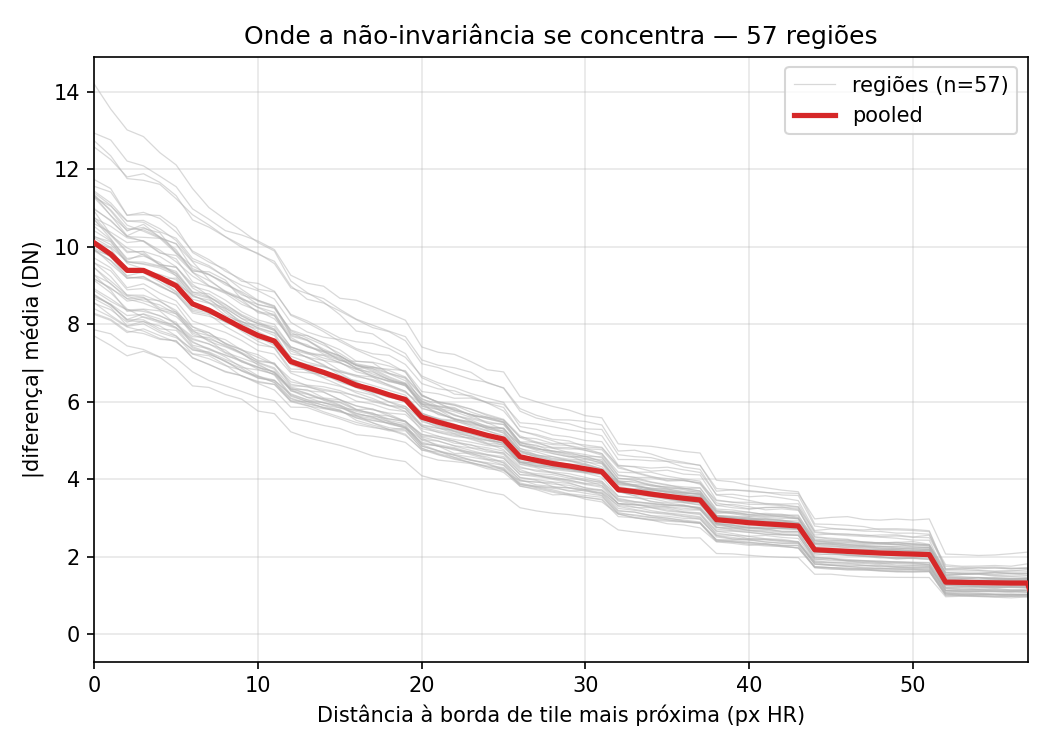
\includegraphics[width=\columnwidth]{fig_border_pooled.png}}
\caption{Perfil de erro vs distância à borda de tile mais próxima (px HR), \emph{pooled}
(57 regiões). A diferença média decai de $\sim$$10{,}1$\,DN na borda para
$\sim$$2{,}0$\,DN no interior, localizando a não-equivariância junto ao
\textit{zero-padding}.}
\label{fig:border}
\end{figure}

\subsection{Comparação de blends}
A Tabela~\ref{tab:blend} e a Fig.~\ref{fig:seam} comparam as estratégias de junção
(\emph{pooled}, média entre as 57 regiões). Sem qualquer \textit{blend} (\texttt{none}),
a costura é nítida: $\mathrm{seam\_excess}=1{,}30$ (excesso de $\sim$30\% de gradiente
nas junções) e PSNR de referência de apenas $25{,}3$\,dB, a manifestação direta do
erro de borda diagnosticado acima. Qualquer ponderação já reduz bastante a costura,
e entre as estratégias clássicas a melhor é a \textbf{gaussiana}, que quase elimina a
costura ($\mathrm{seam\_excess}=1{,}05$) e lidera a fidelidade (PSNR $34{,}4$\,dB,
SSIM $0{,}959$). A máscara \texttt{data-driven} crua ($1{,}09$ /
$32{,}4$\,dB) \emph{não} superou a gaussiana: embora bem fundamentada, o perfil empírico
carrega ruído de amostragem, ao passo que o decaimento suave do peso gaussiano casa bem
com a forma do perfil de erro da Fig.~\ref{fig:border}. Esse resultado sugere
regularizar/parametrizar o perfil antes de usá-lo como máscara, o que motiva as
variantes exploratórias da Tabela~\ref{tab:blendextra}. O \textit{ranking} de blends é
estável entre regiões (desvio-padrão do $\mathrm{seam\_excess}$ ${\sim}0{,}04$ em todas
as estratégias).

\begin{table}[htbp]
\caption{Métricas por estratégia de blend (\emph{pooled}, média entre 57 regiões)}
\label{tab:blend}
\begin{center}
\begin{tabular}{lccc}
\toprule
\textbf{Blend} & \textbf{seam\_excess}$\to 1$ & \textbf{PSNR\_ref}$\uparrow$ & \textbf{SSIM\_ref}$\uparrow$ \\
\midrule
none & 1,303 & 25,26 & 0,697 \\
linear & 1,099 & 32,03 & 0,923 \\
cosine & 1,072 & 33,33 & 0,945 \\
\textbf{gaussian} & \textbf{1,047} & \textbf{34,38} & \textbf{0,959} \\
data-driven & 1,093 & 32,41 & 0,928 \\
\bottomrule
\end{tabular}
\end{center}
\end{table}

\begin{figure}[htbp]
\centerline{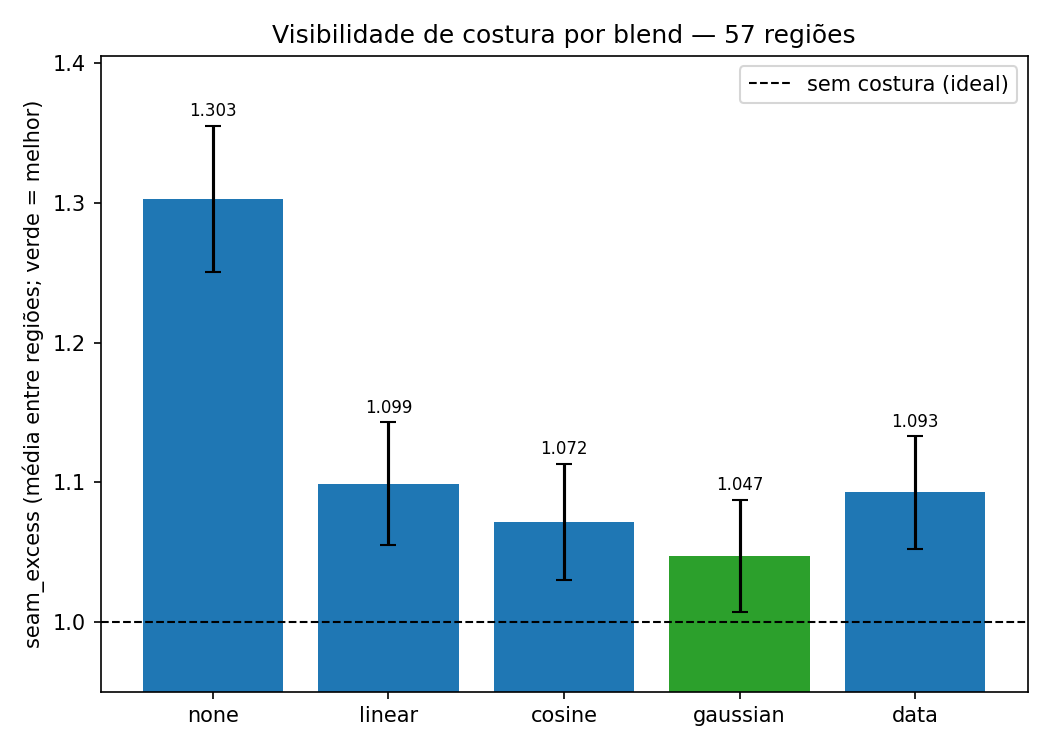
\includegraphics[width=\columnwidth]{fig_blend_pooled.png}}
\caption{Visibilidade de costura ($\mathrm{seam\_excess}$) por estratégia de blend
(\emph{pooled}, 57 regiões); a linha tracejada marca o ideal ($1{,}0$). \texttt{none} é
o pior; \texttt{gaussian} é o mais próximo do ideal entre as clássicas.}
\label{fig:seam}
\end{figure}

\subsection{Discussão}
Os três resultados são coerentes entre si e confirmam a hipótese. (i) A
\textbf{não-equivariância é real e mensurável}: a auto-consistência degrada
monotonicamente com a aproximação às bordas (Tabela~\ref{tab:consistency}). (ii) Sua
\textbf{causa é localizada}: o perfil de borda (Fig.~\ref{fig:border}) mostra que o erro
nasce no \textit{zero-padding} e se propaga pelo campo receptivo excessivo, exatamente
como a teoria de equivariância de CNNs prevê~\cite{b_shiftinv}. (iii) Há um
\textbf{trade-off de junção} bem comportado: ponderar a sobreposição troca um pouco de
nitidez por continuidade, e entre as clássicas o ponto de operação gaussiano domina tanto
a costura quanto a fidelidade. Os três achados se reproduzem com baixa dispersão nas
\textbf{57 regiões}, o que os qualifica como propriedades do gerador, e não de uma área
específica. Na prática, recomenda-se montar mosaicos com \emph{sobreposição
não-nula entre tiles} e \emph{feathering gaussiano}, descartando as bordas onde o erro
de equivariância é máximo; uma sobreposição que cubra a faixa de $\sim$15--20\,px HR de
maior erro já remove a quase totalidade da costura.

\subsection{Estratégias adicionais de junção (exploratório)}
A constatação de que a máscara \texttt{data-driven} crua perde para a gaussiana por
\emph{ruído} de amostragem motiva variantes adicionais, avaliadas com o mesmo protocolo
nas \textbf{57 regiões} (Tabela~\ref{tab:blendextra}). (i) \textbf{Data-driven suavizado}:
ajustando um perfil monótono e suave a $P(d)$ antes de derivar o peso $\propto 1/\hat{P}(d)$,
a máscara guiada por dados passa a \emph{superar} a gaussiana em \emph{todos} os eixos
($\mathrm{seam\_excess}$ $1{,}028$ vs $1{,}047$; PSNR $34{,}85$ vs $34{,}38$\,dB; SSIM
$0{,}964$ vs $0{,}959$) e exibe o \emph{maior} PSNR entre todas as estratégias: a
desvantagem anterior do \texttt{data} cru ($1{,}093$) era de ruído, não de princípio.
(ii) \textbf{Domínio de gradiente (Poisson)}: reconstruindo o mosaico a partir de um campo
de gradientes sem costura (gradiente tomado sempre do tile mais confiável) e resolvendo a
equação de Poisson com condição de \emph{Dirichlet} ancorada ao composto de referência,
obtém-se a \emph{menor} costura ($\mathrm{seam\_excess}=0{,}979$, abaixo de $1$: a junção
fica mais suave que o conteúdo médio) e o \emph{maior} SSIM ($0{,}988$); a Dirichlet ancora
a intensidade e recupera o PSNR para $32{,}4$\,dB (a variante de Neumann derivava o tom e
caía a $\sim$$26$\,dB). (iii) \textbf{Shift-ensemble}: promediar inferências em múltiplos
deslocamentos inteiros explora a \emph{própria} não-equivariância (cada pixel é coberto
por tiles em posições relativas distintas, e os artefatos de borda, dependentes da posição,
se cancelam), atingindo costura quase ideal ($0{,}999$) ao custo de nitidez (PSNR
$28{,}1$; melhor avaliado pela \textit{shift-consistency} que por fidelidade a uma
referência nítida). O gaussiano é, portanto, superado: \emph{Poisson com Dirichlet} domina
costura e estrutura, e o \emph{data-driven suavizado} domina a fidelidade em PSNR.

\begin{table}[htbp]
\caption{Estratégias adicionais vs.\ referência (pooled, 57 regiões; melhores em negrito)}
\label{tab:blendextra}
\begin{center}
\begin{tabular}{lccc}
\toprule
\textbf{Blend} & \textbf{seam\_excess}$\to 1$ & \textbf{PSNR\_ref}$\uparrow$ & \textbf{SSIM\_ref}$\uparrow$ \\
\midrule
poisson (Dirichlet) & \textbf{0,979} & 32,38 & \textbf{0,988} \\
ensemble            & 0,999 & 28,07 & 0,784 \\
smoothed            & 1,028 & \textbf{34,85} & 0,964 \\
gaussian (ref.)     & 1,047 & 34,38 & 0,959 \\
data (cru)          & 1,093 & 32,41 & 0,928 \\
\bottomrule
\end{tabular}
\end{center}
\end{table}

% ===========================================================================
\section{Conclusões}
\label{sec:conclusao}
% ===========================================================================
Medimos, em modo \emph{zero-shot} e sobre Sentinel-2, o grau de (não-)equivariância a
translação do gerador ESRGAN/\texttt{SSR\_RRDBNet} do Satlas. Partindo de uma validação
de região única, estendemos o protocolo a \textbf{57 regiões} e agregamos os resultados
de forma \emph{pooled}. O gerador \textbf{não} é equivariante: a discordância entre
inferências deslocadas do mesmo conteúdo cresce de $30{,}8$ para $24{,}7$\,dB de scPSNR
à medida que a comparação se aproxima das bordas, e o perfil de erro atribui o fenômeno
ao \textit{zero-padding} sob um campo receptivo maior que o tile. Para a montagem de
mosaicos, entre as estratégias clássicas o \textit{blend} gaussiano reduz o excesso de
gradiente nas costuras de $1{,}30$ para $1{,}05$ e eleva o PSNR de referência para
$34{,}4$\,dB, superando a máscara guiada por dados crua; estratégias adicionais (Poisson
com Dirichlet, data-driven suavizado) chegam a superá-lo. \textbf{Todos os achados se
reproduzem com baixa dispersão entre as 57 regiões}, confirmando sua robustez.

\textbf{Limitações e trabalhos futuros.} A validação multi-região realizada (57 áreas
geograficamente distintas) confirmou a robustez do decaimento de borda e do
\textit{ranking} de blends, com baixa dispersão entre regiões. Quatro direções se abrem.
\textbf{(1) Junção em domínio de gradiente:} consolidar a reconstrução de Poisson com
Dirichlet e as máscaras de confiabilidade suavizadas (data-driven regularizado) como
sucessoras da gaussiana. \textbf{(2) Shift-ensemble} como mitigação em tempo de
inferência, avaliada pela própria \textit{shift-consistency} (não só por fidelidade),
estudando o trade-off custo$\times$nitidez com o número de deslocamentos.
\textbf{(3) Anti-aliasing} no gerador (\textit{blur-pool}~\cite{b_shiftinv}) para atacar
a não-equivariância na origem. \textbf{(4) Generalização} a outras tiles/biomas, sensores,
fatores de escala e arquiteturas de SR, testando a universalidade do efeito de borda.
Por fim, o diagnóstico sugere a mitigação direta via \textit{finetuning} com uma perda
explícita de consistência de borda entre tiles deslocados,
\begin{equation}
\mathcal{L}_{borda} = \frac{1}{|\mathcal{B}|}\sum_{(i,j)\in\mathcal{B}}
\bigl\|\nabla I^{SR}_A(i,j) - \nabla I^{SR}_B(i,j)\bigr\|_2,
\label{eq:borda}
\end{equation}
que penalizaria diretamente a discordância de gradiente nas junções, tornando o gerador
mais próximo da equivariância formal de suas camadas.

% ===========================================================================
\begin{thebibliography}{00}

\bibitem{b_esrgan}
X. Wang \textit{et al.}, ``ESRGAN: Enhanced super-resolution generative adversarial
networks,'' in \textit{Proc. ECCV Workshops}, 2018.

\bibitem{b_satlas}
F. Bastani, P. Wolters, R. Gupta, J. Ferdinando, and A. Kembhavi, ``SatlasPretrain: A
large-scale dataset for remote sensing image understanding,'' in \textit{Proc. IEEE/CVF
Int. Conf. Comput. Vis. (ICCV)}, 2023, pp. 16772--16782.

\bibitem{b_satlas_sr}
P. Wolters, F. Bastani, and A. Kembhavi, ``Zooming out on zooming in: Advancing
super-resolution for remote sensing,'' \textit{arXiv preprint arXiv:2311.18082}, 2023.
[Online]. Available: \url{https://arxiv.org/abs/2311.18082}

\bibitem{b_shiftinv}
R. Zhang, ``Making convolutional networks shift-invariant again,'' in
\textit{Proc. ICML}, 2019, pp. 7324--7334.

\bibitem{b_ssim}
Z. Wang, A. C. Bovik, H. R. Sheikh, and E. P. Simoncelli, ``Image quality assessment:
From error visibility to structural similarity,'' \textit{IEEE Trans. Image Process.},
vol. 13, no. 4, pp. 600--612, 2004.

\bibitem{b_lpips}
R. Zhang, P. Isola, A. A. Efros, E. Shechtman, and O. Wang, ``The unreasonable
effectiveness of deep features as a perceptual metric,'' in \textit{Proc. CVPR}, 2018.

\bibitem{b_sr_survey}
Z. Wang, J. Chen, and S. C. H. Hoi, ``Deep learning for image super-resolution: A
survey,'' \textit{IEEE Trans. Pattern Anal. Mach. Intell.}, vol. 43, no. 10,
pp. 3365--3387, 2021.

\bibitem{b_azulay}
A. Azulay and Y. Weiss, ``Why do deep convolutional networks generalize so poorly to
small image transformations?,'' \textit{J. Mach. Learn. Res.}, vol. 20, no. 184,
pp. 1--25, 2019.

\bibitem{b_gconv}
T. S. Cohen and M. Welling, ``Group equivariant convolutional networks,'' in
\textit{Proc. ICML}, 2016, pp. 2990--2999.

\bibitem{b_aliasfree}
T. Karras \textit{et al.}, ``Alias-free generative adversarial networks,'' in
\textit{Proc. Adv. Neural Inf. Process. Syst. (NeurIPS)}, 2021.

\end{thebibliography}

\end{document}
